\documentclass[14pt]{beamer}
\title[JPL:Java:02]{JPL :: Modular Programming - 2}
\author[TS]{TalentSprint}
\institute[L\&D]{Licensed To Skill}
\date{Version 1.0.4}
\usefonttheme{serif}
\usecolortheme{orchid}
\usepackage{bookman}
\usepackage{hyperref}
\usepackage[T1]{fontenc}
\usepackage{graphicx}
\usepackage{listings}
\graphicspath{{Images/} {ScreenShots/}}
\beamertemplateballitem
\usebackgroundtemplate{
\includegraphics[width=\paperwidth]{TS-XP-Logo.jpg}}
\lstset{language=Java,numbers=left, numberstyle=\tiny, basicstyle=\footnotesize, numbersep=10pt, showstringspaces=false, breaklines=true,keepspaces=true, columns=flexible}
\begin{document}

\begin{frame}
  \titlepage
\end{frame}

\begin{frame}{Learning Objectives}
By the end of this presentation, you are able to:
  \begin{itemize}
  \item Write programs to problems by decomposing functionality into methods and using the methods
  \item Write computationally efficient programs
  \item Create meaningful functional decomposition systematically
  \item Develop and test your programs progressively
  \end{itemize}
\end{frame}

\begin{frame}{Modular Programming - 2}
Write a method to check whether or not a number is a Power of two. Using that method, print all 4-digit powers of two.
\end{frame}

\begin{frame}[fragile]{Modular Programming - 2}
Power of Two
\begin{lstlisting}[numbers=none]
public class PowerOfTwo {
    public static void main(String[] args) {
        int i;
        for (i = 1000; i <= 9999; i++) {
            if (isPowerOfTwo (i))
                System.out.println(i + " is power of two");
        }
    }
    public static boolean isPowerOfTwo(int givenNumber) {
        int i;
        for (i = 2; i <= givenNumber; i = i * 2) {
            if (i == givenNumber) 
                return true;
            return false;
        }
    }
}
\end{lstlisting}
\end{frame}

\begin{frame}[fragile]{Modular Programming - 2}
Power of Two - More Configurable
\begin{lstlisting}[numbers=none]
public class PowerOfTwo {
    public static void main(String[] args) {
        int i;
        int n1 = Integer.parseInt(args[0]);
        int n2 = Integer.parseInt(args[0]);
        for (i = n1; i <= n2; i++) {
            if (isPowerOfTwo (i))
	        System.out.println(i + " is power of two");
        }
    }
    public static boolean isPowerOfTwo (int givenNumber) {
        int i;
        for (i = 2; i <= givenNumber; i = i * 2) {
            if (i == givenNumber) 
                return true;
            return false;   
        }
    }
}
\end{lstlisting}
\end{frame}

\begin{frame}[fragile]{Modular Programming - 2}
Power of Two - Different Logic
\begin{lstlisting}[numbers=none]
public static boolean isPowerOfTwo(int givenNumber) {
    while (givenNumber > 1) {
        if (givenNumber % 2 == 1)
            return false;
        givenNumber /= 2;
    }
    return true;
}
\end{lstlisting}
\end{frame}

\begin{frame}{Modular Programming - 2}
\small
\textbf{Why Methods?}

\vspace{1pc}
\begin{minipage}{12cm}
Now, print all the 4-digit Powers of Two with new logic.
\end{minipage}
\begin{minipage}{12cm}
\hspace{5cm}$\downarrow$
\end{minipage}
\begin{minipage}{12cm}
You will find that you do not need to change the main method at all.
\end{minipage}
\begin{minipage}{12cm}
\hspace{5cm}$\downarrow$
\end{minipage}
\begin{minipage}{12cm}
Which logic is better for PowerOfTwo?
\end{minipage}
\end{frame}

\begin{frame}[fragile]{Modular Programming - 2}
\begin{minipage}{7cm}
Write a method to check whether a number is prime or not. 
\end{minipage}
\quad
\begin{minipage}{3cm}

\includegraphics[scale=.4]{exercise.png}
\end{minipage}
\begin{figure}[H]
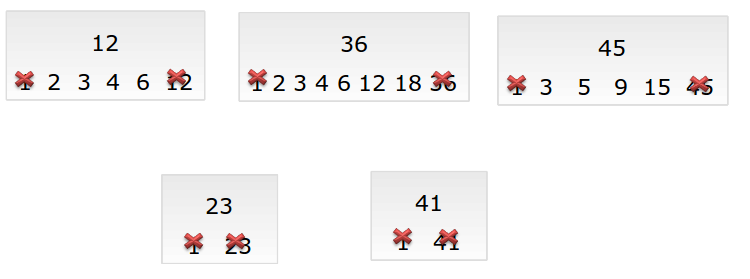
\includegraphics[scale=.4]{modular-programming-prime.png}
\end{figure}
\end{frame}

\begin{frame}[fragile]{Modular Programming - 2}
\begin{lstlisting}[numbers=none]
public class PrimeNumber {
    public static void main(String[] args) {
        int number = Integer.parseInt(args[0]);
        if (isPrime (number))
            System.out.println(number + " is prime");
        else   
            System.out.println(number + " is not prime");
    }
    public static boolean isPrime(int givenNumber) {
        int i;
        for (i = 2; i < givenNumber; i++)
            if (givenNumber % i == 0) 
                return false;
        return true;
    }
}
\end{lstlisting}
\end{frame}

\begin{frame}[fragile]{Modular Programming - 2}
Prime Number - Different Logic
\begin{figure}[H]
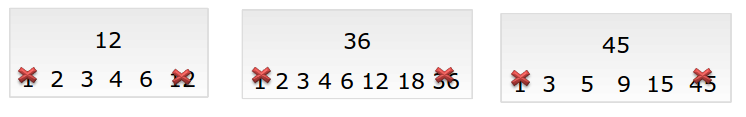
\includegraphics[scale=.4]{prime-logic.png}
\end{figure}
\begin{lstlisting}[numbers=none]
public static boolean isPrime(int givenNumber) {
    int i;
    for (i = 2; i <= givenNumber/2; i++) {
        if (givenNumber % i == 0) 
            return false;
        return true;
    }
}
\end{lstlisting}
\end{frame}

\begin{frame}[fragile]{Modular Programming - 2}
\begin{minipage}{7cm}
Write program that prints prime numbers between 2 and a given number n. 
\end{minipage}
\quad
\begin{minipage}{3cm}

\includegraphics[scale=.4]{exercise.png}
\end{minipage}
\end{frame}

\begin{frame}[fragile]{Modular Programming - 2}
\begin{lstlisting}[numbers=none]
public class PrimeNumberRange {
    public static void main(String[] args) {
        int number = Integer.parseInt(args[0]);
        int i; 	
        for(i = 2; i <= number; i++) {	
            if (isPrime (i))
                System.out.println(number + " is prime");
        }
    }
}
\end{lstlisting}
\end{frame}

\begin{frame}[fragile]{Modular Programming - 2}
\begin{minipage}{7cm}
Write a program to find the aliquot sum of a given number.
\end{minipage}
\quad
\begin{minipage}{3cm}

\includegraphics[scale=.4]{exercise.png}
\end{minipage}
\begin{block}{Hint:}
The aliquot divisors of a number are all of its divisors except the number itself. The aliquot sum is the sum of the aliquot divisors. For example, the aliquot divisors of 12 are 1, 2, 3, 4, and 6 and it's aliquot sum is 16.
\end{block}
\end{frame}

\begin{frame}{Modular Programming - 2}
Let us now explore the modularity a bit more and understand how we can decompose functionality into methods...
\begin{block}{Problem}
Write a program to check whether two given numbers are amicable or not.
\end{block}
\begin{figure}[H]
\begin{center}

\includegraphics[scale=.3]{amicable-thinking.png}
\end{center}
\end{figure}
\end{frame}

\begin{frame}{Modular Programming - 2}
\textbf{Amicable Numbers}

\vspace{1.5pc}
\begin{description}
\item [Aliquot Divisor] Numbers with which a given number gets evenly divided
\end{description}
\end{frame}

\begin{frame}{Modular Programming - 2}
\small
Aliquot Divisors of 284 are: 1, 2, 4, 71 and 142 
\begin{minipage}{12cm}
\hspace{5cm}$\downarrow$
\end{minipage}
Sum of Aliquot Divisors of 284 $\rightarrow$ ASUM(284) 

=  1 + 2 + 4 + 71 + 142  = 220

Aliquot Divisors of 220 are: 
1, 2, 4, 5, 10, 11, 20, 22, 44, 55 and 110
\begin{minipage}{12cm}
\hspace{5cm}$\downarrow$
\end{minipage}
Similarly, the sum of Aliquot Divisors of 220 $\rightarrow$ ASUM(220) 

=  1 + 2 + 4 + 5 + 10 + 11 + 20 + 22 + 44 + 55 + 110  = 284

ASUM(284) = 220 and ASUM(220) = 284

\begin{minipage}{12cm}
\hspace{5cm}$\uparrow$
\end{minipage}
Pair of any numbers in such relation (i.e. ASUM(A)=B and ASUM(B)=A) are called Amicable Pairs.
\end{frame}

\begin{frame}[fragile]{Modular Programming - 2}
Let us write a program to print all 4-digit amicable pairs.

Let us decompose functionality into methods. First, we need a method to find aliquot sum of a given number
\begin{lstlisting}[numbers=none]
public static int  aliquotSum(int n) {
    int i;
    int sum = 1;
    for (i = 2; i <= n/2; i++)
        if ((n % i) == 0)
            sum += i;
    return sum;
}

\end{lstlisting}
\end{frame}

\begin{frame}[fragile]{Modular Programming - 2}
Next, we probably need a method to Find Amicable Pairs - Using \emph{aliquotSum()} Method:
\begin{lstlisting}[numbers=none]
public static boolean areAmicable(int n1,int n2) {
    return ((aliquotSum(n1) == n2) && (aliquotSum(n2) == n1));
}
\end{lstlisting}
\end{frame}

\begin{frame}[fragile]{Modular Programming - 2}
Decomposing functionality into methods

Program to Find Amicable Pairs in a Range:
\begin{lstlisting}[numbers=none]
public static void  amicablePairsInRange (int lower, int upper) {
    int i = lower;
    while (i <= upper ) {
        int j = aliquotSum(i);
        if(i == aliquotSum(j) && j >= i)
            System.out.println("("+i+" , "+j+")"); 
        i++;
    }
}
\end{lstlisting}
\begin{block}{Lesson to Learn:}
Just because we wrote a method, we don't have to use it.
\end{block}
\end{frame}

\begin{frame}[fragile]{Modular Programming - 2}
Decomposing functionality into methods
\begin{block}{Amicable pairs in a range - main:}
\begin{lstlisting}[numbers=none]
class AliquotBad {
    public static void main(String[] args) {
        int n1 = Integer.parseInt(args[0]);
        int n2 = Integer.parseInt(args[1]);
        amicablePairsInRange (n1,n2);
    }	
}
\end{lstlisting}
\end{block}
\end{frame}

\begin{frame}[fragile]{Modular Programming - 2}
Writing Computationally Efficient Programs 
\begin{block}{Program to Find Aliquot Sum:}
\begin{lstlisting}[numbers=none]
public static int  aliquotSum(int n) {
    int i = 2;
    int sum = 1;
    while ( i * i <= n) {
        if ((n % i) == 0)
            sum += i + (n /i);
        i++;
    }
}
\end{lstlisting}
\end{block}
\end{frame}

\begin{frame}[fragile]{Modular Programming - 2}
Writing Computationally Efficient Programs 
\begin{block}{Amicable pairs in a range - main:}
\begin{lstlisting}[numbers=none]
class AliquotGood {
    public static void main(String[] args) {
        int n1 = Integer.parseInt(args[0]);
        int n2 = Integer.parseInt(args[1]);
        amicablePairsInRange (n1,n2);
    }	
}
\end{lstlisting}
\end{block}
\end{frame}

\begin{frame}{Modular Programming - 2}
\begin{block}{Writing Computationally Efficient Programs}
Now, run AliquotBad and AliquotGood, to print all 5-digit amicable pairs, 6-digit amicable pairs and watch the difference.
\end{block}
\end{frame}

\begin{frame}{Modular Programming - 2}
Write a program that prints all Armstrong numbers between two given numbers.
\begin{figure}[H]
\begin{center}
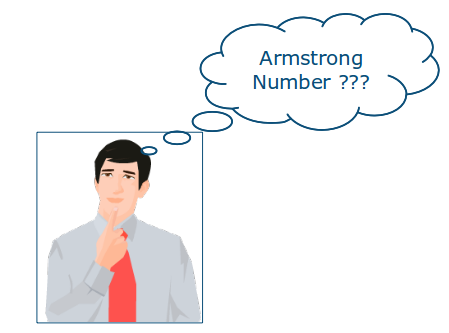
\includegraphics[scale=.4]{armstrong-thinking.png}
\end{center}
\end{figure}
\end{frame}

\begin{frame}[fragile]{Modular Programming - 2}
Armstrong Number
\begin{itemize}
\item A Number of which, each digit is powered by the total digits in the number and summed up and... \item if the sum becomes equal to the original number then the number is called Armstrong Number
\end{itemize}
\begin{verbatim}
          153
      153 ==> 13 53 33
  153 13 53 33 13 + 53  + 33
153 13 53 33 13 + 53  + 33 = 153 
\end{verbatim}
\end{frame}

\begin{frame}[fragile]{Modular Programming - 2}
\small
Making Meaningful Functional Decomposition
\begin{block}{Problem}
Writing a program that prints all Armstrong numbers between two given numbers.
\end{block}
\begin{description}
\item [Step 1] At the highest level, we need to loop through each number between the two given numbers
\item [Step 2] Check if it is Armstrong Number
\item [Step 3] If it is, print it.
\end{description}
Looping and printing can be done by \textbf{main()} method. Checking can be done by another method called \emph{isArmstrong()}.
\end{frame}

\begin{frame}[fragile]{Modular Programming - 2}
\small
Making Meaningful Functional Decomposition
\begin{block}{Problem}
Writing \emph{isArmstrong()} method
\end{block}
\begin{description}
\item [Step 1] It requires us to find Sum of Powers of Digits.
\item [Step 2] First, we can have a method to find digits of the given number. Let's call it \emph{getDigits()}.
\item [Step 3] Let's have another method that finds sum of powers for the given digits. Let's call it \emph{sumOfPowers()}.
\end{description}
So, we will have four methods namely: main, isArmstrong, getDigits, sumOfPowers.
\end{frame}

\begin{frame}[fragile]{Modular Programming - 2}
\begin{block}{Code for \emph{getDigits()} Method:}
\begin{lstlisting}[numbers=none]
public static int[] getDigits(int number) {
    int[] digits = new int[Integer.toString(number).length()];
    int index=0;
    while (number > 0) {
        digits[index++] = number % 10;
        number = number / 10;
    }
    return digits;
}
\end{lstlisting}
\end{block}
\end{frame}

\begin{frame}[fragile]{Modular Programming - 2}
\begin{block}{Let us test \emph{getDigits()} first}
\begin{lstlisting}[numbers=none]
public static void main(String args[]) {		
    int digits[];
    int givenNum = Integer.parseInt(args[0]);
    digits [] = getDigits(givenNum);
    for (int i = 0; i < digits.length; i++)
        System.out.println(digits[i]);
}
\end{lstlisting}
\end{block}
\end{frame}

\begin{frame}[fragile]{Modular Programming - 2}
\begin{block}{Code for \emph{sumOfPowers()} Method:}
\begin{lstlisting}[numbers=none]
public static int sumOfPowers(int[] digits) {
    int sum = 0;
    int length = digits.length;
    for(int counter = 0; counter < length; counter++)
        sum += Math.pow(digits[counter], length);
    return sum;
}
\end{lstlisting}
\end{block}
\end{frame}

\begin{frame}[fragile]{Modular Programming - 2}
\begin{block}{Now, let us test \emph{sumOfPowers}}
\begin{lstlisting}[numbers=none]
public static void main(String args[]) {		
    int numDigits[];
    int givenNum = Integer.parseInt(args[0]);
    numDigits [] = getDigits(givenNum);
    int sum = sumOfPowers(numDigits);
    System.out.println(sum);
}
\end{lstlisting}
\end{block}
\end{frame}

\begin{frame}[fragile]{Modular Programming - 2}
\begin{block}{Code for \emph{isArmstrong()} Method:}
\begin{lstlisting}[numbers=none]
public static boolean isArmstrong(int number) {		
    int numDigits[];
    numDigits [] = getDigits(number);
    int sumPowers = sumOfPowers(numDigits);
    return (number == sumPowers);
}
\end{lstlisting}
\end{block}
\end{frame}

\begin{frame}[fragile]{Modular Programming - 2}
\begin{block}{Code for \textbf{main()} Method:}
\begin{lstlisting}[numbers=none]
public static void main(String args[]) {
    int startNum = Integer.parseInt(args[0]);
    int endNum = Integer.parseInt(args[1]);
    for(int i = startNum; i <= endNum; i++)
        if (isArmstrong(i))
            System.out.println(i+ "   ");	
}
\end{lstlisting}
\end{block}
\end{frame}

\begin{frame}[fragile]{Modular Programming - 2}
\small
For the following problems, use a separate method that takes line number (n) as a parameter and returns 'n'th line as a string. The main method calls that method iteratively to print one line at a time. 

\begin{enumerate}
\item Write a program which accepts a number as argument and print the following output. The pyramid shape should be preserved for 2-digit numbers as well.
\begin{verbatim}
    Input : 5
    Output: 
              1
            1 2
          1 2 3
        1 2 3 4 
      1 2 3 4 5
\end{verbatim}
\end{enumerate}
\end{frame}

\begin{frame}[fragile]{Modular Programming - 2}
\begin{enumerate}
\setcounter{enumi}{1}
\item Write a program which accepts a number (number of lines) and character as arguments and print the following output. 
\begin{verbatim}
    Input : 5, %
    Output : 

             %
           %   %
          %  %  %
         %  %   %  %
        %  %  %  %  %
\end{verbatim}
\end{enumerate}
\end{frame}

\begin{frame}{Modular Programming - 2}
\begin{block}{Problem}
Write a program that finds the least number that can be formed using the digits of the given number.
\end{block}
\begin{description}
\item [Step 1] Get the digits of the given number. (getDigits method)
\item [Step 2] Sort the digits. (sort method)
\item [Step 3] Form the number with the sorted digits.  (getNumberFromDigits method)
\end{description}
\end{frame}

\begin{frame}[fragile]{Modular Programming - 2}
\begin{block}{Code for \emph{getDigits()} Method:}
\begin{lstlisting}[numbers=none]
public static int[] getDigits(int number) {
    int[] numDigits = new int[Integer.toString(number).length()];
    int index=0;
    while(number > 0) {
        numDigits[index++] = number % 10;
        number = number / 10;
    }
    return numDigits;
}
\end{lstlisting}
\end{block}
\end{frame}

\begin{frame}[fragile]{Modular Programming - 2}
\textbf{Arays.sort()} method is available in Java which sorts an array. Now, we need another method for generating the number from sorted digits.
\begin{block}{Code for generating number from digits}
\begin{lstlisting}[numbers=none]
public static int getNumberFromDigits(int[] digits) {
    int theNumber = 0;
    for (int i = 0; i < digits.length; i++)
        theNumber = theNumber * 10 + digits[i];
    return theNumber;
}
\end{lstlisting}
\end{block}
\end{frame}

\begin{frame}[fragile]{Modular Programming - 2}
Then, we will have the main method using all the methods.
\begin{lstlisting}[numbers=none]
public static void main(String args[]) {
    int givenNum = Integer.parseInt(args[0]);
    int[] digits = getDigits(givenNum);
    Arrays.sort(digits);
    int leastNum = getNumberFromDigits(digits);
    System.out.println ("The least no. is : " + leastNum);
}
\end{lstlisting}
\end{frame}

\begin{frame}{Modular Programming - 2}
Can we do without using sort? 
\begin{enumerate}
\item We know that all digits are between 0 and 9. 
\item So, parse the digits of the given number few times. 
\item In the first pass, find and copy all 0's. 
\item In the second pass, find all 1's, then all 2's and so on until all 9's. 
\item Then, form the number from the copied digits.
\end{enumerate}
\end{frame}

\begin{frame}[fragile]{Modular Programming - 2}
\begin{block}{Code for parsing the digits}
\begin{lstlisting}[numbers=none]
public static int[] parseDigits(int[] origDigits) {
    int[] parsedDigits = new int[origDigits.length];
    int i, j, index = 0;
    for (i = 0; i <= 9; i++)
        for (j = 0; j < origDigits.length; j++)
            if (origDigits[j] == i)            
                parsedDigits[index++] = i;
    return parsedDigits;
}
\end{lstlisting}
\end{block}
\end{frame}

\begin{frame}[fragile]{Modular Programming - 2}
\begin{minipage}{7cm}
Write the main method now using the \emph{parseDigits()} method instead of \textbf{Arrays.sort()}.

Analyze which approach is better. 
\end{minipage}
\quad
\begin{minipage}{3cm}

\includegraphics[scale=.4]{exercise.png}
\end{minipage}
\end{frame}

\begin{frame}{Modular Programming - 2}
 \begin{figure}[H]
 \begin{center}
   
\includegraphics[scale=.3]{qa.png}   
 \end{center}
  \end{figure}
\end{frame}
\end{document}
